\documentclass[linenumbers,RNAAS,trackchanges]{aastex631}
\usepackage[utf8]{inputenc}
\usepackage{hyperref}           % hrefs
\usepackage{natbib}             % for bibliography
\usepackage{float}              % figure positioning
\usepackage{svg}                % used for SVG images
\usepackage{graphicx}           % used for non-SVG images
\usepackage{csvsimple}
\usepackage{listings}

% Search Query Metadata
\shorttitle{Lagrange Points for the Sun-Jupiter System}
\shortauthors{Ajaykumar, et al.}

% Hyperlink setup
\hypersetup{
colorlinks=true,
linkcolor=blue,
urlcolor=blue
}

\begin{document}
\title{Calculation of the Location and Stability of the Five Lagrange Points and Simulation of the Sun-Jupiter system}
% [] is for ORCiD
\correspondingauthor{}
\email{nikhitaajaykumar@utexas.edu, khernandez@utexas.edu, darryl.tran@utexas.edu}
\author{Nikhita Ajaykumar}

\author{Kayla Hernandez}

% or 
% \nocollaboration{0}

\author{Darryl Tran}
\affiliation{University of Texas at Austin\\
110 Inner Campus Drive\\
Austin, TX 78705}

% 250 word limit for abstract
\begin{abstract}
The Lagrange Points are five positions in space where a relatively smaller-massed object in a system of two massive orbiting bodies can be placed to maintain its position while orbiting. Conceptually, the gravitational forces of the two bodies equal the centripetal force of a smaller object required for it to move along with the bodies. This phenomenon is an incredible tool for agencies around the world as man-made satellites and telescopes are sent into space to study natural phenomena in the universe. This paper will explore methods used to determine the five Lagrange points and their stability in the Sun-Jupiter system.
\end{abstract}

% Use astrothesaurus numbers in place of num
\keywords{Lagrange (1) --- Classical Mechanics (2) --- Celestial Bodies (3)}
\section{Introduction} \label{sec:intro}
In 1867, Newton first defined the three-body problem in his work “Philosophiæ Naturalis Principia Mathematica”. Since then, the classical three-body problem has challenged scientists to the present day and The attempts at solving the problem through various methods have led to the discovery of Neptune, the location and stability of the Trojan asteroids, and variants of the problem are used in quantum mechanics for analysis on various elements. The problem has also greatly expanded our collective knowledge of the stability of the solar system. The three body problem produces the conceptual context for the study of classical dynamics and different areas of mathematics (calculus, geometry, linear algebra).\cite{unknown}


Although the three body problem's open solution remains unsolved, several scientists have come up with special case solutions. In the 1760s, Euler found several periodic solutions to the three-body problem in which the three bodies are collinear at each moment. In 1772, Lagrange found a group of solutions in which the three bodies form an equilateral triangle at each instant. In this special case solution, the three bodies were assumed to be a restricted system, meaning that the mass of the first two celestial bodies is much greater than the third celestial body. Lagrange’s solutions, together with Euler’s solutions form the central configuration of the three-body problem. The Lagrangian solutions are not referred to as the Lagrangian points: L1, L2, L3, L4, and L5.\cite{unknown}


The L1 and L2 points of the Sun-Earth systems are important points for NASA missions. SOHO (Solar and Heliospheric Observatory) is parked at L1. The L2 point was the home of WMAP (Wilkinson Microwave Anisotropy Probe), currently homes PLANCK, and is the future home of the James Webb Space Telescope. Currently, there is minimal use of the L3 point. The L4 and L5 are points in which Trojan asteroids orbit. The name Trojans comes from the three  asteroids Agamemnon, Achilles, and Hector that orbit in the L4 and L5 points of the Jupiter-Sun system. Understanding the location and stability of these points can provide potential landing spots for various space missions. This paper will be focused on finding the 5 Lagrangian points in the Sun-Jupiter system and elucidating the stability of these points.\cite{unknown}
 



\newpage
\section{Problem to be Solved} \label{sec:problem}
\begin{center}Equations to determine X and Y coordinates for the Lagrange points:\end{center}
\begin{equation}
\label{eqn:"Eq. 1"}
0 = -\frac{GM_\odot(x + R_\odot)}{((x + R_\odot)^2 + y^2)^\frac{3}{2}} - \frac{GM_J(x - R_{J})}{((x - R_{J})^2 + y^2)^\frac{3}{2}} + \omega^2x 
\end{equation}

\begin{equation}
\label{eqn:"Eq. 2"}
0 = -\frac{GM_\odot y}{(x + R_\odot)^2 + y^2)^\frac{3}{2}} - \frac{GM_{J} y}{((x - R_{J} )^2 + y^2)^\frac{3}{2}} + \omega^2y
\end{equation}

where $G = \SI{6.67408e-11}{\frac{m^3}{kg.s^2}}, M_\odot = \SI{1.9891e30}{kg}, R_\odot = \SI{-7.4e8}{m}, M_{J} = \SI{1.898e27}{kg}, R_{J} = \SI{7.77e11}{m}, $and $\, {\omega} = \SI{1.66e-8}{s^{-1}}.$ Here, ${\omega}$ refers to the angular velocity of Jupiter as it orbits the Sun.

These equations are derived by using center of mass,
$$M_1 r_1 + M_2 r_2 = 0,$$
angular velocity,
$$\omega = \frac{2\pi}{P},$$
and Kepler's 3rd Law,
$$(M_1 +M_2) P^2 = \frac{4\pi^2}{G}a^3$$ where $a$ is the semi-major axis.

If we let $\omega^2 = \frac{G(M_1 + M_2}{(r_1 -r_2)^3}$, then we can get

$$\frac{GM_1}{(x+r_1)^2} + \frac{GM_2}{(x-r_2)^2} = \omega^2r$$ for the Lagrange point on the left hand side of the larger mass. Then to find the Lagrange point in the area between the two masses,

$$\frac{GM_1}{(x+r_1)^2} + \frac{GM_2}{(x+r_2)^2} = -\omega^2r.$$
Finally, the L2 point on the right hand side of the lesser mass can be analytically solved using

$$\frac{GM_1}{(x+r_1)^2} - \frac{GM_2}{(x-r_2)^2} = \omega^2r.$$

For the last two Lagrange points the equation 

$$\frac{M_1}{S^3}(r - r_1) + \frac{M_2}{S^3}(r-r_2) = \frac{(M_1+M_2)r}{|r_1 - r_2|^3}$$ can be used since L4 and L5 are equidistant from the two masses and a reflection of each other across the x-axis. 

\section{Data} \label{sec:data}
The Secant method of determining roots was used to determine three Lagrange points. For points L1, L2, and L3, the y-variable of \ref{eqn:"Eq. 1"} and \ref{eqn:"Eq. 2"} was set to 0 due to these points being aligned with the Sun and Jupiter in a straight line. By setting the y-variable to 0, the system of two equations was reduced to a system of one equation and the Secant method was used to determine the roots of the equation. The method requires two bounds to iteratively find the roots. The bounds were determined by plotting the equation and identifying regions where x would cross zero. The secant method requires two bounds to iteratively find the roots. The bounds were determined by plotting the equation and identifying regions where x would cross zero. The graphs below correspond to different Lagrange points and are labeled accordingly (see: Secant Method for Computing L1, L2, and L3 in Appendix for code).

L4 and L5 were found using a modified  Newton-Rhapson method for nonlinear systems of equations. The partial differential equations for \ref{eqn:"Eq. 1"} and \ref{eqn:"Eq. 2"}  in respect to x and y were found using the sympy python library. These partial differentials were inputted into a Jacobian matrix and were used within the modified Newton-Raphson computation to find the roots of the multi-variable system. We compared this value to the exact computation (see: Information about Observations for mathematical proof of L4 and L5 points), and found a 0.3 percent error (see: Modified Newton-Raphson Method for L4 and L5 Computation for code).



Furthermore, a stability analysis was performed to complement the calculation of each Lagrange point. Other literature have agreed that points L1 to L3 are relatively unstable while points L4 and L5 enjoy stable equilibrium. This topic will be discussed further in later sections. 

\begin{figure}[H]
    \centering
    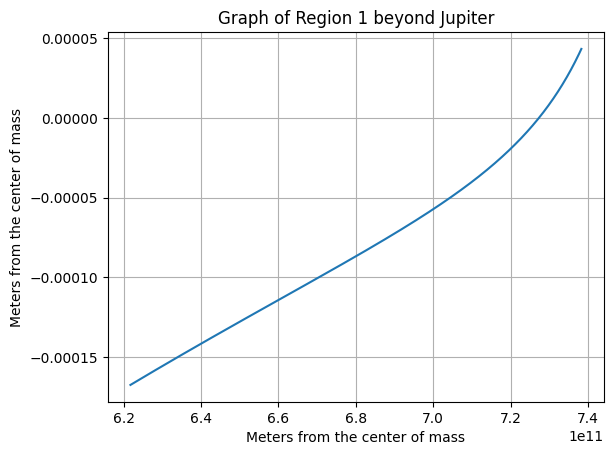
\includegraphics[scale=.75]{l1.png}
    \caption{Graph of Region 1, from Jupiter to deep space)}
    \label{fig:asa}
    \centering
    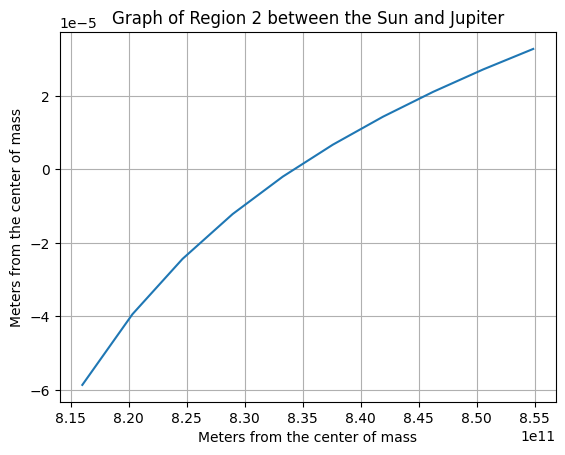
\includegraphics[scale=.75]{l2.png}
    \caption{Graph of Region 2, from the Sun to Jupiter}
    \label{fig:code}
\end{figure}

\begin{figure}
    \centering
    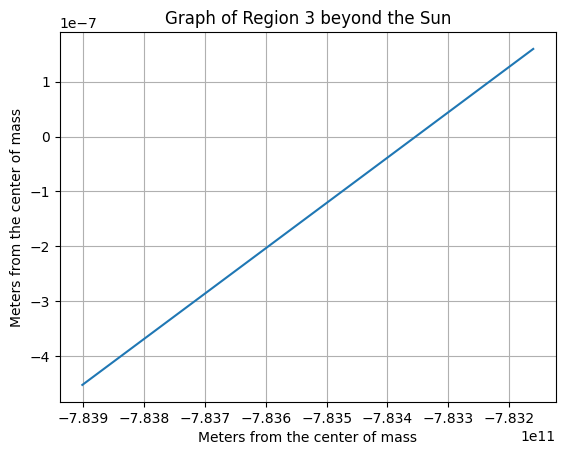
\includegraphics[scale=.75]{l3.png}
    \caption{Graph of Region 3, from the Sun into deep space}
    \label{fig:code}
\end{figure}


\begin{table}[H]
\centering
\csvautotabular[respect all]{lagrange.csv}
\caption{Coordinates of the calculated Lagrange points along with their associated error}
\end{table}


\newpage
\section{Information about Observations}\label{sec:observations}

\begin{figure}[H]
    \centering
    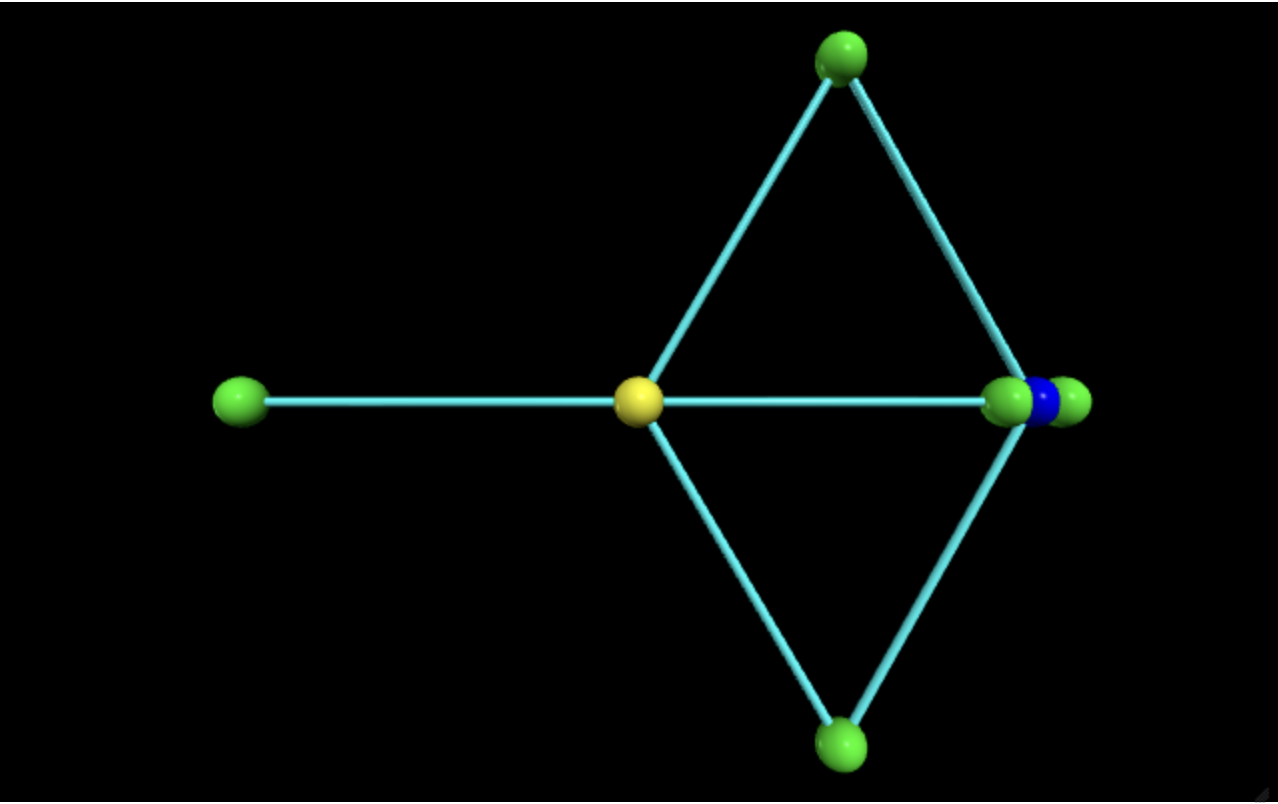
\includegraphics[scale=.75]{lagrangepoints.png}
    \caption{Lagrange points for Sun Jupiter system modeled using Vpython}
    \label{fig:code}
\end{figure}

With the L4 and L5 points found, we can prove that an equilateral triangle is formed between the coordinates of the Sun, Jupiter, and the two points. By definition, an equilateral triangle contains two properties. An equilateral triangle must have three equal sides and three equal angles. 

One side is already known, the distance between the Sun and Jupiter is approximately 5.2 AU or $7.779e11$ meters. The distance between L4 and either mass can be calculated with the distance formula $d = \sqrt{(x_2 - x_1 )^2 + (y_2 - y_1) ^ 2}$ where $x_2$ and $y_2$ refer to the coordinates of L4 and $x_1$ and $y_1$ refer to the coordinates of the Sun or Jupiter respectively. The distance between L4 and the Sun in AU is $d_{L4-R_\odot} \approx 5.2 AU$ while the distance between L4 and Jupiter is $d_{L4-R_{J}} \approx 5.2AU$. This satisfies the first property of equilateral triangles where all sides must be equal. 

With the sides or distances between the points now known, proving the second property is trivial. Since each side is equal to each other where $d_{{\odot}-{J}}$ = $d_{L4-R_\odot}$ = $d_{L4-R_{J}}$, it follows that there must be three equal angles thus satisfying the second property and proves that the three points form an equilateral triangle. 

Calculations using the same logic when proving $\triangle {L4}{\odot}{J}$ is equilateral provides similar results for the triangle formed by L5, the Sun, and Jupiter. 

\newpage
\section{Stability Analysis} \label{sec:Stability analysis}
According to Neil J. Cornish, L1 and L2 are unstable as they have a positive real eigenvalue produced from the linearized equations of motion matrix. Both are saddle points. If a satellite was placed at either of these points, it would wander off within months. L3 also has a positive real eigenvalue and thus is unstable. L4 and L5 are points of interest because they will have purely imaginary eigenvalues, and thus would be stable, if

$$k^2 \geq \frac{23}{27}$$ and $$\sqrt{27k^2 - 23} \leq 2$$

where $k = (M1 - M2) / (M1 + M2)$. In the case of the Sun and Jupiter, these two equations are satisfied.\cite{cornish_1998}


\section{Conclusion} \label{sec:conclusion}
The methods of computation and derivations referenced in this paper successfully computed the location and stability of the 5 Lagrangian points in the Sun-Jupiter system. Through the stability analysis, it is discovered the L1, L2, and L3 points lack proper stability, meaning fuel will need to be used by the spacecraft to stay at any of the collinear points. The L4 and L5 points are stable. The stability of the L4 and L5 points demonstrates why Trojan asteroids accumulate at the L4 and L5 points. At these points, a spacecraft could be landed and left without fuel used to provide stability. Even small perturbations of the spacecraft would be stabilized. It is necessary to note that the Cornish paper used to understand the stability of each Lagrange point is not a peer-reviewed article.\cite{westra}

There are several ways to expand this problem. Examining the effects of the gravitation force from closer large bodies like Saturn on the calculation of the Lagrange points would provide a more accurate picture of the location and stability of the 5 Lagrange points. Jupiter also has 4 moons (Io, Europa, Ganymede, and Callisto). These moons are relatively large and also could also exert some gravitational force on the Lagrange points and could form their own Lagrange points with Jupiter, although the gravitation forces of each moon on the orbit of the other moon would destabilize the points. 

\section{Appendix} \label{sec:appendix}

\begin{center} \textbf{Python Libraries:} \end{center}

\begin{lstlisting}[language=Python]
import numpy as np
import numpy.linalg as la
import matplotlib.pyplot as plt
from matplotlib import cm
import math
import scipy.optimize
import math
from sympy import *
\end{lstlisting}

\begin{center} \textbf{Constants:} \end{center}

\begin{lstlisting}[language=Python]
G = 6.67408e-11
standard_mass = 1.9891e30
m_sun = 1.9891e30
r_sun = 6.957e8
m_jupiter = 1.89813e27
revolution_jupiter = 4333 * 24 * 3600
omega_jupiter = 2 * np.pi / (3.784e8)
r_jupiter = 7.4115e11
AU = 1.496e11
R_sun = -741629000
oopsies = 4.5e7
R_jupiter = (7.779e11+R_sun)
\end{lstlisting}
\newpage
\begin{center} \textbf{Secant Method for Computing L1, L2, and L3:} \end{center}

\begin{lstlisting}[language=Python]
def secant (f, a, b, tol):
    # f is differentiable function
    # a and b are close approximations to the root
    # tol is the tolerance

    # Use an approximation for the derivative
    # f_prime(x_n) = (f(x_n) - f(x_n -1)) / (x_n - x_n-1)
    prev_x = (b + a) / 2
    x = b
    while abs(f(x)) > tol:
        f_prime = (f(x) - f(prev_x))/(x - prev_x)

        # Obtain a better approximation
        # x_n+1 = x_n - (f(x_n))/ f_prime(x_n)
        prev_x, x = x, x - (f(x))/f_prime
    # repeat until f(x_n) is less than the tolearnce
    return x
\end{lstlisting}

\begin{center} \textbf{Modified Newton-Raphson Method for L4 and L5 Computation:} \end{center}

\begin{lstlisting}[language=Python]
#equations
X, Y = symbols ('X Y')
f0 = -((G * m_sun * (X + R_sun)/ ((X + R_sun)**2 + Y **2) **(3/2))) - (((G * \
        m_jupiter) * (X - R_jupiter)/ ((X - R_jupiter)**2 + Y**2) **(3/2))) + \ 
        omega_jupiter **2 * X 
f1 = -((G * m_sun * Y/ ((X + R_sun)**2 + Y**2) **(3/2))) - (((G * m_jupiter) \ 
* Y/ ((X - R_jupiter)**2 + Y **2) **(3/2))) + omega_jupiter **2 * Y
a = diff(f0, X)
#print(a)
b = diff(f0, Y)
#print(b)
c = diff(f1, X)
#print(c)
d = diff(f1, Y)
#print(d)


def newton(F, J, x, tol):
    F_value = F(x)
    F_norm = np.linalg.norm(F_value, ord=2) 
    
    while abs(F_norm) > tol:
        dx = np.linalg.solve(J(x), -F_value)
        x = x + dx
        F_value = F(x)
        F_norm = np.linalg.norm(F_value, ord=2)
 
    return x


def L4_L5():
    def F(x): #ax and ay equations
        return np.array([-((G * m_sun * (x[0] + R_sun)/ ((x[0] + R_sun)**2 \
        + x[1] **2) **(3/2))) - (((G * m_jupiter) * (x[0] - R_jupiter)/ \
        ((x[0] - R_jupiter)**2 + x[1]**2) **(3/2))) + omega_jupiter **2 * x[0], \
        -((G * m_sun * x[1]/ ((x[0] + R_sun)**2 + x[1]**2) **(3/2))) - (((G * m_jupiter) \ 
        * x[1]/ ((x[0] - R_jupiter)**2 + x[1] **2) **(3/2))) + omega_jupiter **2 * x[1]])

    def J(x): #jacobian matrix of partial differentials found using sympy
        return np.array([[-2.13045032403201e-36*(3.86021705735445e-12 - \
        4.96709190996342e-24*x[0])*(1.26682714704e+17*x[0] - 9.84525321932184e+28)/ \
        (1.65569730332114e-24*x[1]**2 + (1.28673901911815e-12*x[0] - 1)**2)**2.5 
        - (2224887000.0 - 3.0*x[0])*(1.3275412528e+20*x[0] - 9.84543091772811e+28)/(x[1]**2 + (x[0] - 741629000)**2)**2.5 - 2.69891230590392e-19/(1.65569730332114e-24*x[1]**2 + (1.28673901911815e-12*x[0] - 1)**2)**1.5 \
        - 1.3275412528e+20/(x[1]**2 + (x[0] - 741629000)**2)**1.5 + 2.75713150761897e-16, \ 
        1.05821425690784e-59*x[1]*(1.26682714704e+17*x[0] - 9.84525321932184e+28)/ \ 
        (1.65569730332114e-24*x[1]**2 + (1.28673901911815e-12*x[0] - 1)**2)**2.5 + \ 
        3.0*x[1]*(1.3275412528e+20*x[0] - 9.84543091772811e+28)/(x[1]**2 + \ 
        (x[1] - 741629000)**2)**2.5], [-2.69891230590392e-19*x[1]*(3.86021705735445e-12 - \ 
        4.96709190996342e-24*x[0])/(1.65569730332114e-24*x[1]**2 +  \ 
        (1.28673901911815e-12*x[0] - 1)**2)**2.5 - 1.3275412528e+20*x[1]*(2224887000.0 - \ 
        3.0*x[0])/(x[1]**2 + (x[0] -  741629000)**2)**2.5,1.34057454803561e-42*x[1]**2/ \ 
        (1.65569730332114e-24*x[1]**2 + (1.28673901911815e-12*x[0] - 1)**2)**2.5 +  \ 
        3.9826237584e+20*x[1]**2/x[1]**2 + (x[0] - 741629000)**2)**2.5 - \ 
        2.69891230590392e-19/(1.65569730332114e-24*x[1]**2 + \ 
        (1.28673901911815e-12*x[0] - 1)**2)**1.5 - \ 
        1.3275412528e+20/(x[1]**2 + (x[0] - 741629000)**2)**1.5 + 2.75713150761897e-16]])


    tol = 1e-6
\end{lstlisting}
\begin{center} \textbf{Sun-Jupiter Visualization:} \end{center}

\begin{lstlisting}[language=Python]
from vpython import *

# define constants
G  = 6.674e-11 # Universal gravitational constant [N m^2 kg^-2]

# radius of the sun (not to scale)
# r_sun = 6.9634e8
R_sun = 5e10

# radius of jupiter(not to scale)
# r_jup = 6.6854e7
R_jup = 5e10

M_sun   = 1.9891e+30  # Solar mass [kg]
M_jup = 1.898e27      # Jupiter mass [kg]
d_sj = 7.4e8 + 7.77e11 # distance between sun and Jupiter

sun = sphere (pos=vector(-741629000,0,0), radius = R_sun, color = color.yellow, \ 
make_trail = True)
jupiter = sphere (pos=vector(7.779e11,0,0), radius = R_jup, color = color.blue, \ 
make_trail = True)

# initalize jupiter's velocity
jupiter.velocity = vector (0,8e3,0)

# initalize sun's velocity
sun.velocity = vector(0, -5e1, 0)


# Lagrange points
L1 = sphere(pos = vector (727.2979800351156e9, 0, 0), radius = 5e10, color = color.green)
L2 = sphere(pos = vector (834.2214601529249e9, 0, 0), radius = 5e10, color = color.green)
L3 = sphere(pos = vector (-783.3440958825038e9, 0, 0), radius = 5e10, color = color.green)
L4 = sphere(pos = vector (398.6630666379343e9, 675.5019899267185e9, 0), radius = 5e10, \ 
color = color.green)
L5 = sphere(pos = vector (398.6630666379343e9, -675.5019899267185e9, 0), radius = 5e10, \ 
color = color.green)
l1 = curve(pos = [vector(0,0,0), vector (727.2979800351156e9, 0, 0)], radius = 1e10, \ 
color = color.cyan)
l2 = curve(pos = [vector(0,0,0), vector (834.2214601529249e9, 0, 0)], radius = 1e10, \ 
color = color.cyan)
l3 = curve(pos = [vector(0,0,0), vector (-783.3440958825038e9, 0, 0)], radius = 1e10, \ 
color = color.cyan)
l3_s = curve(pos = [vector(7.779e11,0,0), vector (-783.3440958825038e9, 0, 0)], \ 
radius = 1e10, color = color.cyan)
l4 = curve(pos = [vector(0,0,0), vector (398.6630666379343e9, 675.5019899267185e9, 0)], \ 
radius = 1e10, color = color.cyan)
l4_s = curve([vector(7.779e11,0,0), vector (398.6630666379343e9, 675.5019899267185e9, 0)], \ 
radius = 1e10, color = color.cyan)
l5 = curve(pos = [vector(0,0,0), vector (398.6630666379343e9, -675.5019899267185e9, 0)],\ 
radius = 1e10, color = color.cyan)
l5_s = curve(pos = [vector(7.779e11,0,0), vector (398.6630666379343e9, \
-675.5019899267185e9, 0)], radius = 1e10, color = color.cyan)


\end{lstlisting}



\newpage
\bibliographystyle{ieeetr}
\bibliography{citation}


\section{Acknowledgements} \label{sec:acknowledgements}
We would like to express our gratitude to Brett Barkley and Dr. Shyamal Mitra for their guidance, lectures, and multiple extensions. 

We would also like to extend our gratitude to Neil J. Cornish for his derivations on the stability of the five Lagrange points.  

\end{document}

\end{document}
